\chapter{Ceph Distributed Storage System}\label{chap:ceph} 
Ceph uniquely delivers object, block, and file storage in one unified system. Ceph is highly reliable, easy to manage, and free. Ceph delivers extraordinary scalability–thousands of clients accessing petabytes to exabytes of data. A Ceph Node leverages commodity hardware and intelligent daemons, and a Ceph Storage Cluster accommodates large numbers of nodes, which communicate with each other to replicate and redistribute data dynamically

\section{Motivation}\label{sec:ceph_motivation}
 Prior to Ceph, storage infrastructures were typically built using multiple specialized systems. Traditional solutions often required centralized metadata management or separate systems for block, file, and object storage—leading to inefficiencies and increased costs. The motivation behind Ceph was to consolidate these diverse storage needs into one cohesive system that:
\begin{itemize}
    \item \textbf{Delivers Unified Storage:} By integrating object, block, and file interfaces, Ceph simplifies infrastructure management.
    \item \textbf{Enhances Scalability:} Ceph is designed to scale out by using a distributed algorithm (CRUSH) for data placement, which eliminates central bottlenecks. 
    \item \textbf{Ensures High Availability:} Its self-healing and self-managing properties allow for automatic data replication and recovery, ensuring continuous operation despite hardware failures.
\end{itemize}
These goals were driven by the need for a flexible, resilient system that could serve modern cloud and big data applications without resorting to expensive, specialized hardware. \cite{cloudification2024} 

\section{Challenges}\label{sec:ceph_challenges}
Designing a distributed storage system like Ceph involves addressing several core challenges: 

\begin{itemize}
    \item \textbf{Data Placement and Scalability:} Distributing data across thousands of nodes requires a robust algorithm (such as CRUSH) that dynamically balances loads and adapts to changes in the cluster. 
    \item \textbf{Fault Tolerance and Self-Healing:} The system must detect and recover from node or disk failures automatically, ensuring data durability without manual intervention. 
    \item \textbf{Performance Optimization:} Achieving high throughput and low latency across a network of commodity hardware is complex, especially when replicating or erasure-coding data. 
    \item \textbf{Heterogeneous Hardware Support:} Supporting a mix of storage devices (HDDs, SSDs, NVMe) while maintaining consistent performance requires careful tuning and design. 
    \item \textbf{Management Complexity:} The distributed nature of the system introduces challenges in configuration, monitoring, and scaling, all of which must be simplified for operational efficiency. 
\end{itemize}

\section{Ceph Architecture}

\subsection{Core Components}

Ceph's architecture is built around the following key components:

\begin{itemize}
    \item \textbf{Object Storage Device (OSD) Daemons}: These are the primary storage nodes responsible for storing and replicating data. Each OSD runs as a separate daemon on a physical or virtual storage device.
    \item \textbf{Monitors (MONs)}: MONs maintain the cluster map and manage metadata, ensuring that all clients and OSDs have a consistent view of the system.
    \item \textbf{Managers (MGRs)}: A Ceph Manager serves as an endpoint for monitoring, orchestration, and plug-in modules.
    \item \textbf{Metadata Servers (MDSs)}: Used for CephFS, these servers handle file system metadata and allow POSIX-compliant access to data.
\end{itemize}

Storage cluster clients and Ceph OSD Daemons use the CRUSH algorithm to compute information about the location of data. By using the CRUSH algorithm, clients and OSDs avoid being bottlenecked by a central lookup table. \cite{ceph_architecture}

\subsection{Cluster Maps and Topology Changes}

Ceph's architecture relies on various maps to represent the cluster's state:

\begin{itemize}
    \item \textbf{Monitor Map}: Lists all active MONs.
    \item \textbf{OSD Map}: Details all OSDs and their statuses.
    \item \textbf{Placement Group (PG) Map}: Describes the distribution of PGs across OSDs.
    \item \textbf{CRUSH Map}: Defines the data placement rules using the CRUSH algorithm, determining how data is distributed across the cluster.
\end{itemize}

When the cluster topology changes, such as adding or removing OSDs, these maps are updated to reflect the new state, ensuring that data placement and access remain consistent.

\subsection{Data Storage Workflow}

Ceph organizes data through a hierarchical structure:

\begin{enumerate}
    \item \textbf{Files}: User data is initially in file form.
    \item \textbf{Objects}: Files are divided into objects for storage.
    \item \textbf{Pools}: Objects are grouped into pools, which are logical collections that manage replication and placement rules.
    \item \textbf{Placement Groups (PGs)}: Pools are subdivided into PGs, which act as intermediaries to distribute objects evenly across OSDs.
    \item \textbf{OSDs}: PGs map to OSDs where the actual data resides.
\end{enumerate}

This structure ensures efficient data distribution and management within the cluster.

\subsection{Role of Placement Groups}

Placement Groups aggregate objects into manageable units, facilitating balanced data distribution and simplifying replication processes. By mapping multiple objects to a single PG, Ceph reduces the complexity of tracking individual object locations, enhancing scalability and performance.
\begin{enumerate}
    \item \textbf{Efficient Data Management}: By grouping objects, PGs reduce the complexity of tracking individual objects, enhancing performance.
    \item \textbf{Optimized Data Distribution and Recovery}: PGs enable even data distribution across OSDs. In case of an OSD failure, entire PGs can be replicated or moved, ensuring swift recovery and data integrity.
\end{enumerate}

\begin{figure}[h]
    \centering
    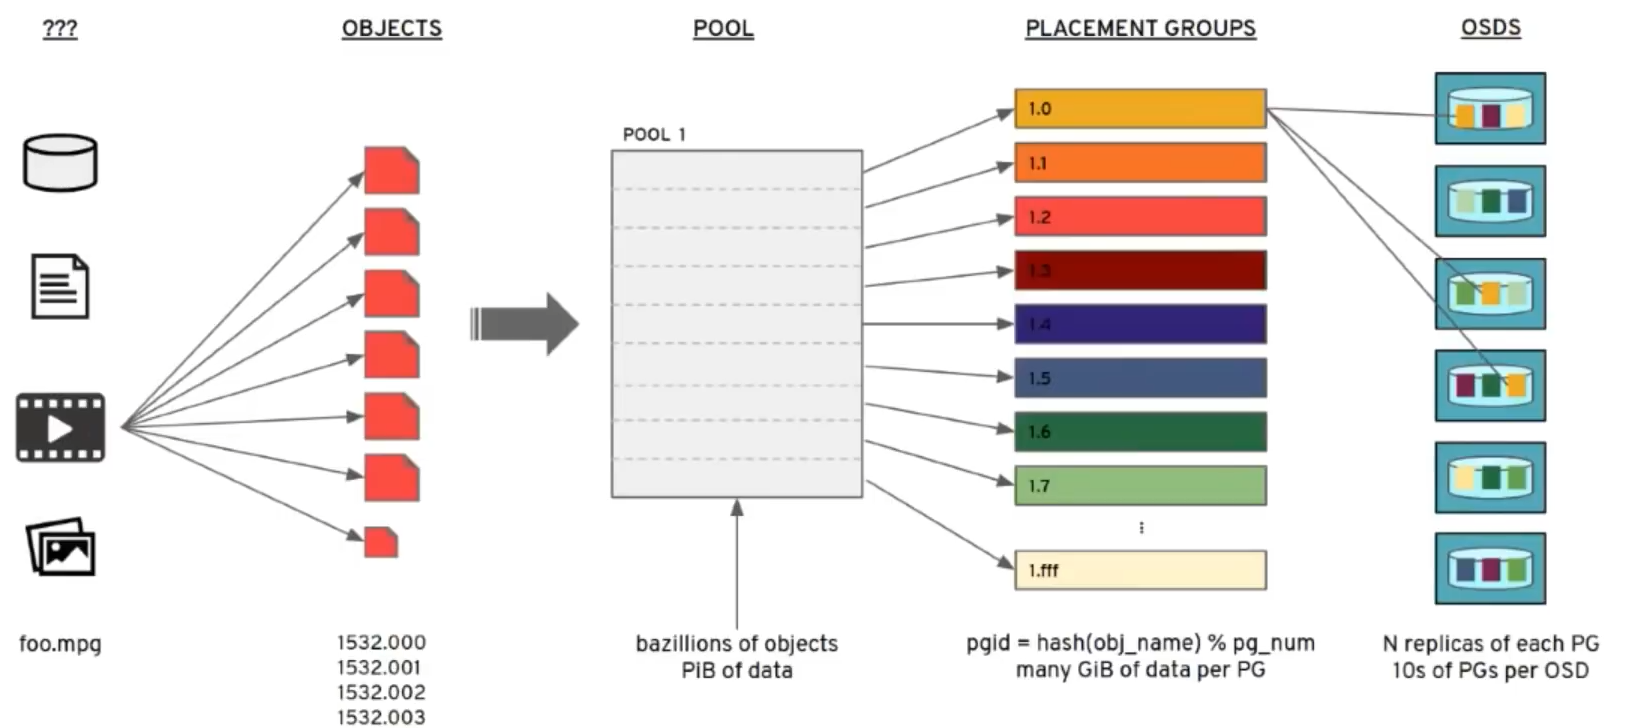
\includegraphics[width=0.8\textwidth]{img/obj_pg_osd.png}
    \caption{Relation between File, Objects, Placement Groups and OSDs. Source:  \cite{ceph_intro_video}.} 
    \label{fig:obj_pg_osd}
\end{figure}

\subsection{Data Protection Mechanisms}

Ceph employs two primary methods to ensure data durability:
\begin{itemize}
    \item \textbf{Replication}: Each object is copied to multiple OSDs based on predefined replication factors. This approach ensures data availability even if some OSDs fail.
    \item \textbf{Erasure Coding}: Data is split into chunks and encoded with redundancy information. This method provides fault tolerance with reduced storage overhead compared to replication.
\end{itemize}
\begin{figure}[h]
    \centering
    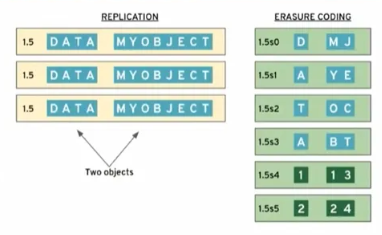
\includegraphics[width=0.7\textwidth]{img/replication_erasure_coding.png}
    \caption{Comparison of replication and erasure coding techniques \cite{ceph_intro_video}.}
    \label{fig:replication_erasure}
\end{figure}

  

\subsection{RADOS Gateway (RGW)}

The RGW is an object storage interface that provides RESTful APIs compatible with Amazon S3 and OpenStack Swift, enabling applications to interact with Ceph's object storage seamlessly.

\subsection{RGW Federation and Geo-Replication}

To enhance scalability and disaster recovery, Ceph's RGW supports:

\begin{itemize}
    \item \textbf{Federation}: Distributes the workload across multiple zones, allowing for scalable and efficient data access.
    \item \textbf{Geo-Replication}: Asynchronously replicates data across geographically dispersed clusters, ensuring data availability and disaster recovery.
\end{itemize}

\subsection{Metadata Server (MDS)}

For the Ceph File System (CephFS), the MDS manages metadata operations, such as directory structures and file attributes. This separation of data and metadata operations allows Ceph to handle high metadata workloads efficiently, providing POSIX-compliant file system access.
